\section{Klassifikationsergebnis von Rasa NLU (Fabio Aubele)}\label{anhang:nlu}
In diesem Anhang ist das erzielte Klassifikationsergebnis des neuronalen Netzes von Rasa NLU als Konfusionsmatrix zu sehen. Auf der linken Achse sind dabei die korrekten Labels der einzelnen Äußerungen aufgelistet, wohingegen auf der unteren Achse die vorhergesagten Labels zu finden sind. Dies bedeutet, dass alle richtig bestimmten Labels auf der Diagonalen liegen, was hier bei den meisten Testdaten der Fall ist. Die Farbe der Kästchen gibt an, wie oft das Beispiel aufgetreten ist. Der Intent 'tell\_art\_and\_artist' tritt dabei am meisten auf, da dieser für alle der drei Gesprächsfälle aus Kapitel \ref{sec:dialog} verwendet wird und nur durch die Angabe der Entities die verschiedenen Fälle unterschieden werden.
\begin{figure}[htbp]
	\centerline{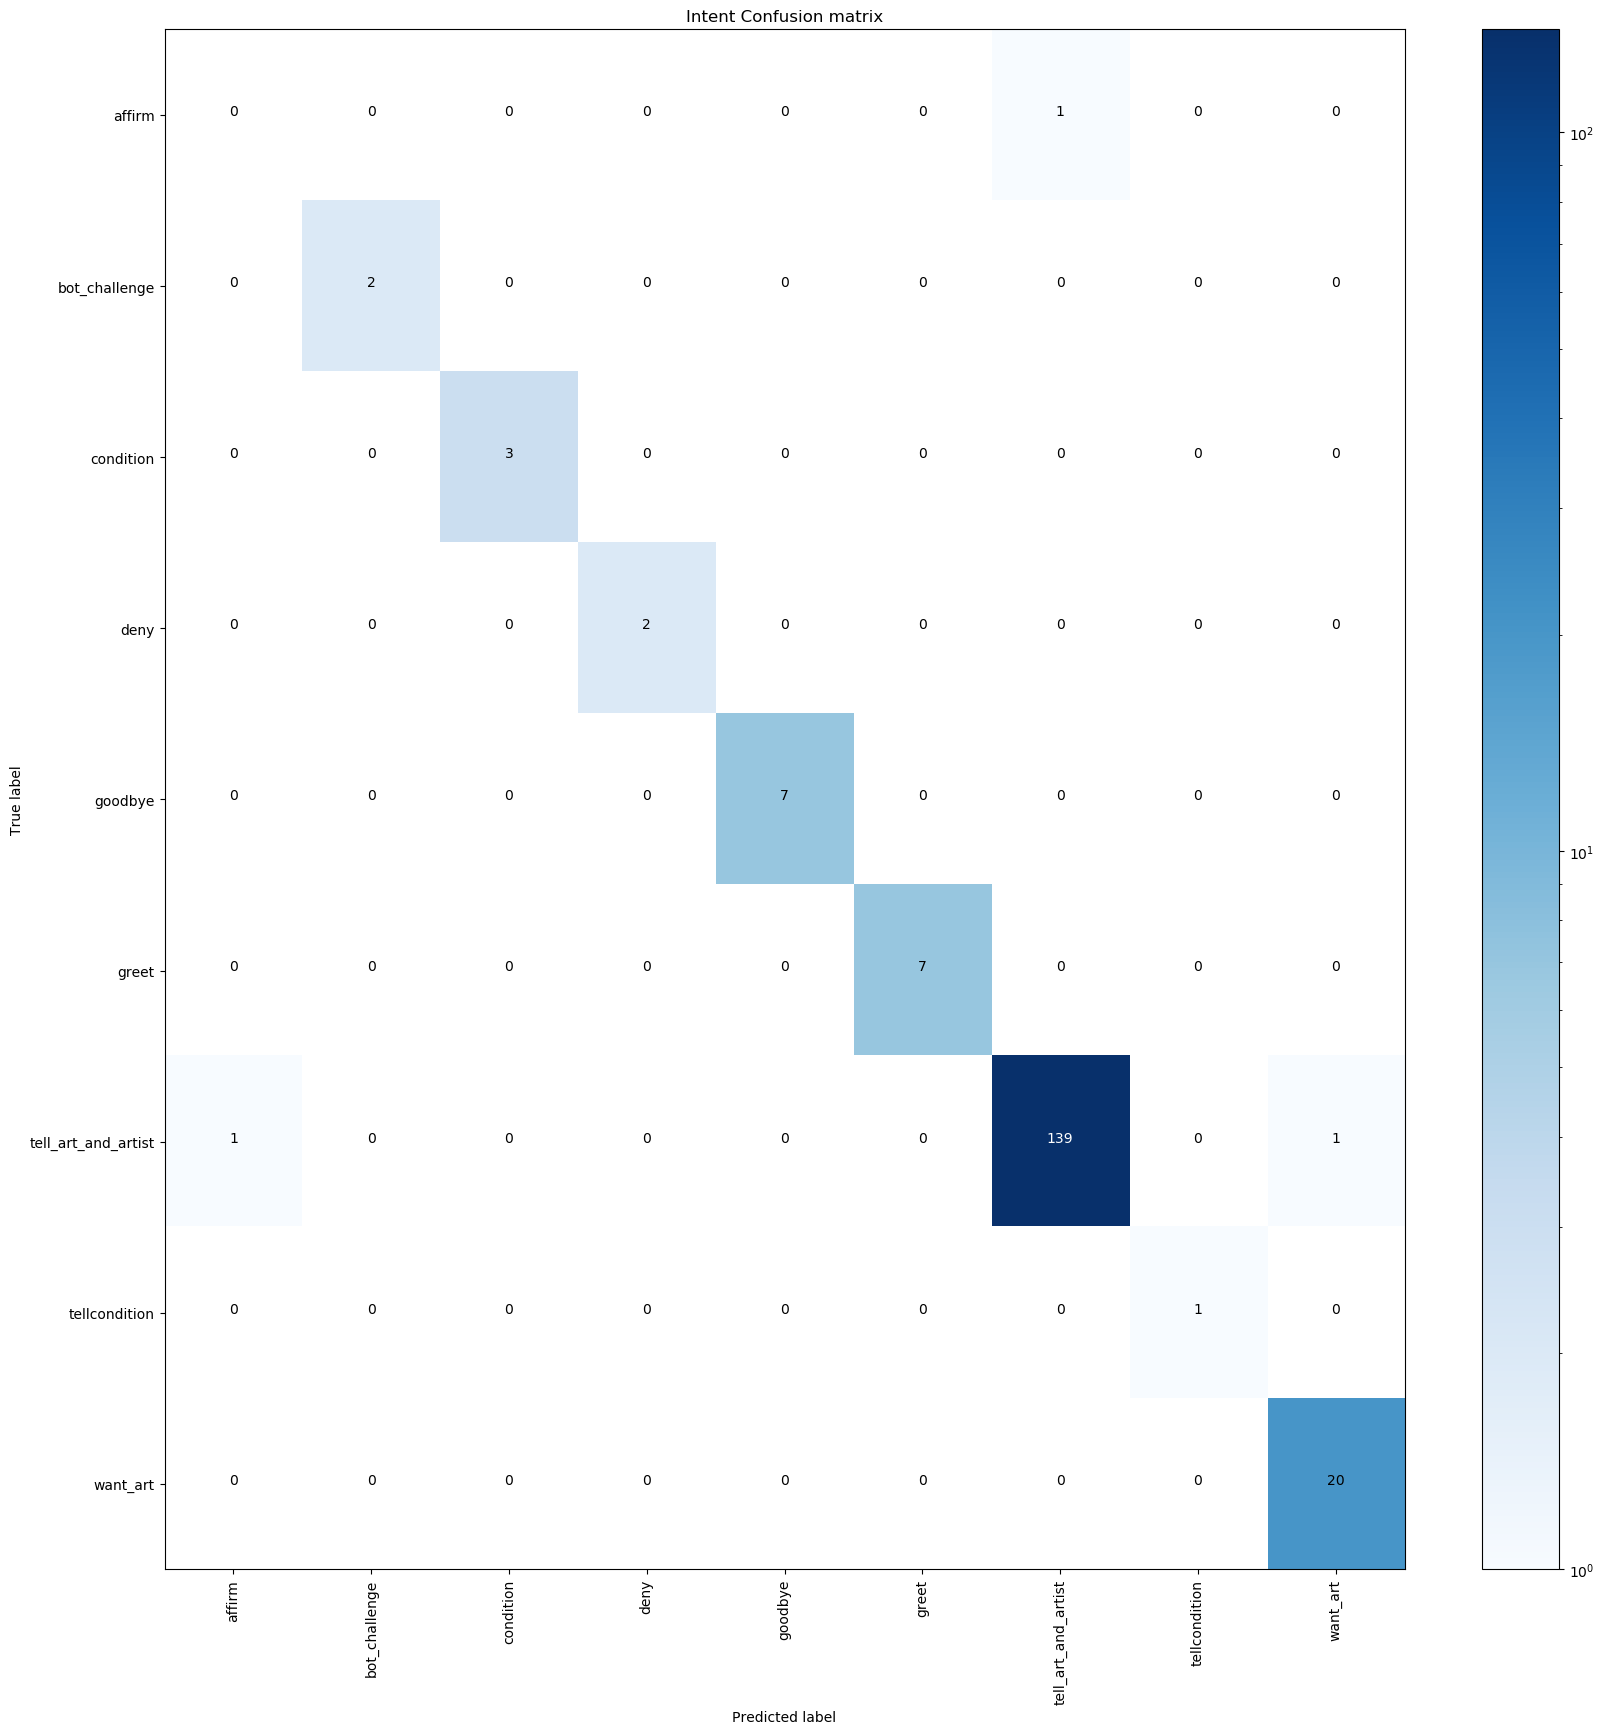
\includegraphics[width=1\linewidth]{figures/confmat.png}}
	\caption{Konfusionsmatrix des Klassifikationsergebnis von Rasa NLU.}
	\label{confnlu}
\end{figure}

\newpage

\section{Klassifikationsergebnis von Rasa Core (Fabio Aubele)}\label{anhang:core}
Dieser Anhang stellt das Klassifikationsergebnis von Rasa Core dar. Der Aufbau ist dabei derselbe wie bei Rasa NLU (Anhang \ref{anhang:nlu}). Jedoch sind die Labels auf den Achsen hierbei die entsprechenden Antworten des Chatbots, welche von dem neuronalen Netz bestimmt wurde. Am meisten tritt dabei 'action\_listen' auf, da diese Aktion immer ausgelöst wird, wenn der Chatbot eine neue Eingabe erwartet. Um alles vollständig lesen zu können, muss das Dokument eventuell etwas vergrößert werden, wenn es in digitaler Form vorliegt.
\begin{figure}[htbp]
	\centerline{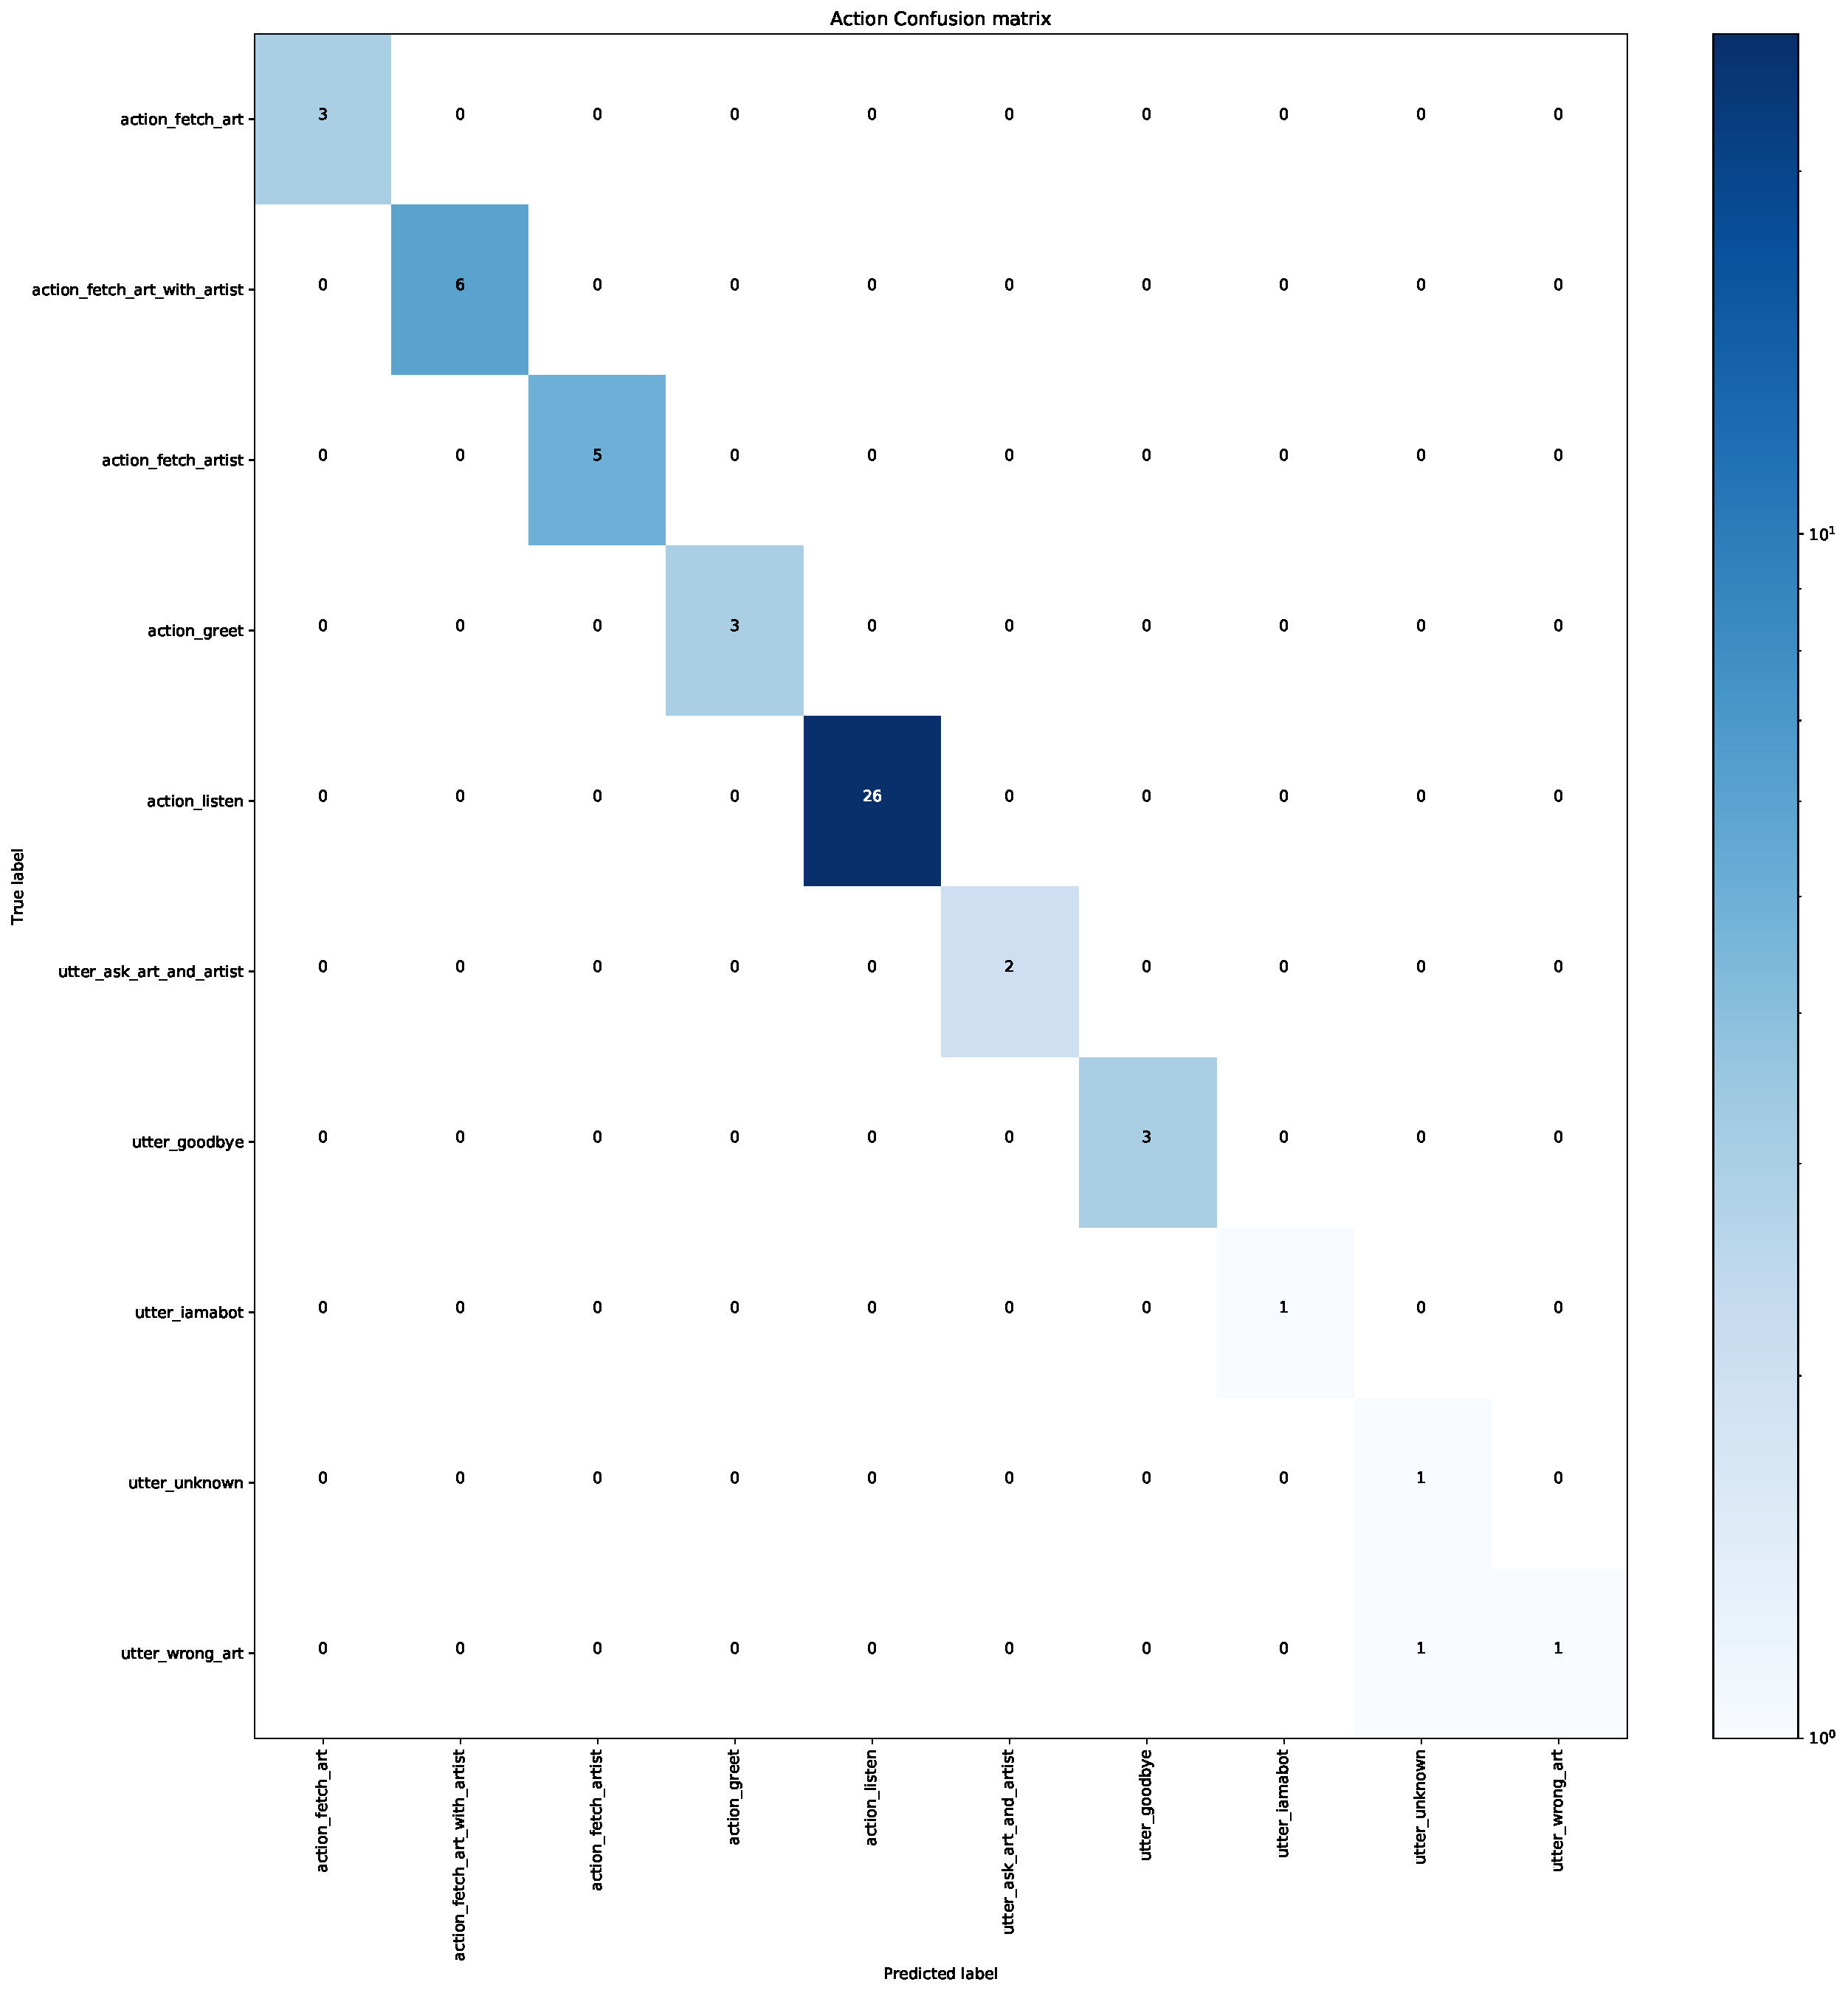
\includegraphics[width=1\linewidth]{figures/story_confmat.pdf}}
	\caption{Konfusionsmatrix des Klassifikationsergebnis von Rasa Core.}
	\label{confcore}
\end{figure}